This chapter provides an overview of the \ac{DT} concept,
its historical development and the more recent models and technologies that have emerged
to support its implementation.
%
The ever-growing literature on the subject reflects the increasing interest in \acp{DT}
and its multi-faceted nature, encompassing various domains and applications.
%
In this thesis we focus on the software engineering perspective of \acp{DT}, 
and the application of \acp{DT} to the engineering of \ac{IoT} systems.
%
Accordingly, this chapter focuses on how the \ac{DT} concept has been interpreted in this context.


%=======================================================
\section{History and Definitions}
%=======================================================

The concept of \ac{DT} was introduced in the early 2000s by Michael Grieves
in the context of Product-Lifecycle Management~\cite{Grieves_2023}
where it was conceived as a virtual representation of a product throughout its lifecycle.
%
At its essence, Grieves defined what later came to be known as a \ac{DT} as a system composed of three main components (\Cref{fig:dt-grieves-original}):
\begin{itemize}
\item a \emph{physical space} and its products;
\item a \emph{virtual space} containing the digital representation of the products;
\item a \emph{connection} between the two, making data flow from the physical to the virtual space and information flow from the virtual to the physical space~\cite{Grieves2017}.
\end{itemize}

\begin{figure}[ht]
    \centering
    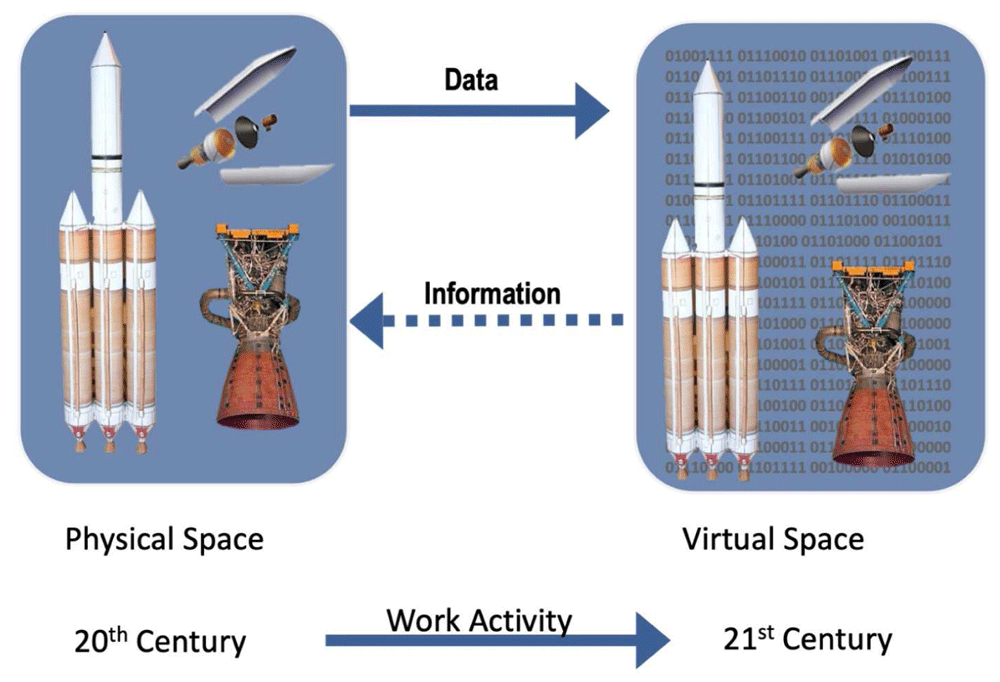
\includegraphics[width=0.7\textwidth]{figures/dt-original.png}
    \caption{The original \ac{DT} model by Grieves, from \cite{Grieves_2022}.}
    \label{fig:dt-grieves-original}
\end{figure}

Grieves referred to this concept as the \emph{Mirrored Spaces Model}~\cite{Grieves_2005},
a name which echoes the idea of \emph{Mirror Worlds} introduced by David Gelernter in the 1990s~\cite{gelernter1991mirrorworlds}
who also envisioned the ability to replicate the real world in a completely virtual space~\cite{Singh_Fuenmayor_Hinchy_Qiao_Murray_Devine_2021}.

The idea was later associated with its modern \emph{\acl{DT}} name and popularized by NASA in the 2010s, when it was presented as a key technology
for future development of aircraft and spacecraft in order to virtually simulate extreme conditions,
integrate data from the physical system in operation, 
and provide feedback on the conditions of the \emph{flying twin}
while possibly enacting changes to mitigate damage~\cite{glaessgen2012dtnasa}.
%
NASA's definition hence focused on the ability of the \ac{DT} to integrate multiple simulation models and characterized the \ac{DT} as \emph{ultra-realistic}, as the goal was to virtually replicate the physical system with the highest possible degree of fidelity:

\begin{quote}
    A Digital Twin is an integrated multiphysics, multiscale, probabilistic simulation of an as-built vehicle or system that uses the best available physical models, sensor updates, fleet history, etc., to mirror the life of its corresponding flying twin~\cite{glaessgen2012dtnasa}.
\end{quote}

Given the various phases of a product's lifecycle, the \ac{DT} concept was later
refined to distinguish between the \emph{Digital Twin Prototype} (DTP) and the \emph{Digital Twin Instance} (DTI) and \emph{Digital Twin Aggregate} (DTA)~\cite{Grieves2017}.
The DTP is the virtual representation of the product during its design and development phase,
while the DTI is the virtual representation of the product during its operational phase.
%
The DTA represents instead the aggregation of all DTIs, hence all products that have been built~\cite{Grieves_2022}.
%
Interestingly, the DTP exists before the physical product is even produced, 
and it is rather ``just'' a virtual model of the product. 
%
Grieves argues that requiring that a \ac{DT} exists only when the physical product exists is a \emph{fallacy}~\cite{Grieves_2022}.
%
Nevertheless, it is generally accepted within the community nowadays that, for a proper characterization, what is usually referred as \ac{DT} is hence a DTI, which exists alongside its physical counterpart and is continuously updated with data from the physical world. 

The role of such bidirectional data exchange between the physical and virtual parts
of a \ac{DT} has been, in fact, used to characterize the \ac{DT} concept and distinguish it from other related concepts.
%
A widely accepted taxonomy classifies the concepts of \emph{Digital Model}, \emph{Digital Shadow} and \emph{Digital Twin} based on direction of the automatic data flow between the physical and virtual spaces~\cite{kritzinger2018dtmanufacturing} (\Cref{fig:dt-taxonomy}):
namely, 
a Digital Model (\Cref{fig:dt-taxonomy-digital-model}) is a static model of a physical system (similarly to the DTP) that can be manually updated over time,
the Digital Shadow (\Cref{fig:dt-taxonomy-digital-shadow}) gets automatically updated through an inbound data flow from the physical space,
while the Digital Twin (\Cref{fig:dt-taxonomy-digital-twin}) is the only one that holds a bidirectional data flow which can provide feedback to the physical counterpart.
%
Such connection has been referred to as the \emph{digital thread}~\cite{Singh_Willcox_2018,Grieves_2023} to evoke the idea of a tie that binds the physical and virtual spaces.
%
Other common terms include \emph{twinning}~\cite{JONES202036} or \emph{shadowing}~\cite{Jiang_Yin_Li_Luo_Kaynak_2021,web-of-dt-ricci-2022} process. 
%
This terminology emphasizes the continuous and dynamic nature of the relationship between the physical and virtual entities, 
and highlights the active role of such process in maintaining the \ac{DT} up to date.

\begin{figure}[ht]
    \centering
    \begin{subfigure}[b]{0.3\linewidth}
        \centering
        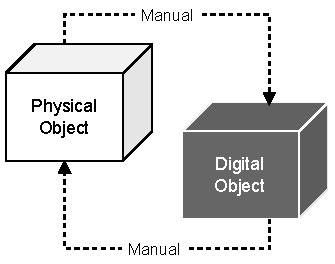
\includegraphics[width=\linewidth]{figures/kritzinger-digital-model.pdf}
        \caption{Digital Model}
        \label{fig:dt-taxonomy-digital-model}
    \end{subfigure}
    \hfill
    \begin{subfigure}[b]{0.3\linewidth}
        \centering
        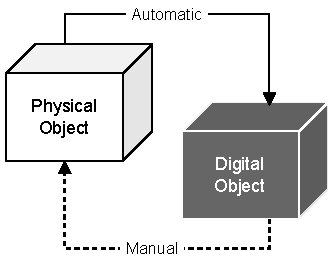
\includegraphics[width=\linewidth]{figures/kritzinger-digital-shadow.pdf}
        \caption{Digital Shadow}
        \label{fig:dt-taxonomy-digital-shadow}
    \end{subfigure}
    \hfill
    \begin{subfigure}[b]{0.3\linewidth}
        \centering
        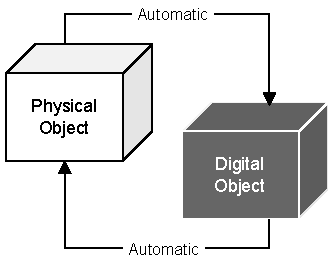
\includegraphics[width=\linewidth]{figures/kritzinger-digital-twin.pdf}
        \caption{Digital Twin}
        \label{fig:dt-taxonomy-digital-twin}
    \end{subfigure}
    \caption{Taxonomy of Digital Twin related concepts based on the data flows between physical and digital objects, adapted from \cite{kritzinger2018dtmanufacturing}.}
    \label{fig:dt-taxonomy}v
\end{figure}

The scope and applicability of the \ac{DT} concept has evolved and expanded
to encompass a wide range of applications and domains.
%
Today, \acp{DT} are used in various fields such as manufacturing, healthcare, smart cities, and more.
%
This is also reflected in the abundance of terminology used to identify the physical counterpart of a \ac{DT}
which is nowadays often referred to as the \emph{physical twin} or
\emph{physical entity}~\cite{Singh_Fuenmayor_Hinchy_Qiao_Murray_Devine_2021,JONES202036,DBLP:journals/jss/DaliborJRSWWW22}.
%
This shift from identifying the physical counterpart as a \emph{product} to a more generic \emph{entity}
highlights the broader applicability of the \ac{DT} concept beyond its original manufacturing context.
%
The \ac{DT} concept has been adopted also to represent people~\cite{Shengli_2021},
processes (e.g., supply chain~\cite{Barykin_Bochkarev_Kalinina_Yadykin_2020}) and organizations~\cite{Parmar_Leiponen_Thomas_2020}, leading to a more abstract interpretation of what can be considered \emph{physical}. 
%
Accordingly, the definitions of \acp{DT} have also diversified, leading to a plethora of interpretations~\cite{DBLP:journals/jss/DaliborJRSWWW22}. 

For the scope of this thesis, 
since the focus is on how \acp{DT} can be used to engineer \ac{IoT} systems, taking as the reference context the healthcare domain,
we adopt the following definition, adapted from \cite{dt-IoT-context-Minerva-2020}:

\begin{quote}
A \acf{DT} is a comprehensive software representation of an individual \acl{PA}.
It includes the properties, conditions, and behavior(s) of the real-life asset through models and data.
A \ac{DT} is a set of realistic models that can simulate an asset's behavior in the deployed environment.
The \ac{DT} represents and reflects its physical twin and remains its virtual counterpart across the asset's entire lifecycle.
\end{quote}

The definition emphasizes the software nature of the \ac{DT} and its ability to model the properties and behavior of its physical counterpart.
%
We deliberately use the term \emph{\ac{PA}} to refer to the physical counterpart of a \ac{DT}
to highlight the fact that an \emph{asset} is something that has a strategic
value in the context of an application domain, and that the \ac{DT} is meant to represent and manage such assets.
%
Compared to the original Grieves model which characterized the \ac{DT} as having three parts (physical, digital and connection), for the reminder of this thesis we will instead consider:
\begin{itemize}
\item the \ac{PA} as the physical counterpart of a \ac{DT};
\item the \ac{DT} as the software implementing the virtual representation of the \ac{PA} through a combination of models and data;
\item the \emph{twinning process} implemented by the \ac{DT} software to keep the \ac{DT} up to date with the \ac{PA} and possibly provide feedback to it.
\end{itemize}

%=======================================================
\section{Reference Architectures and Properties}
%=======================================================

The conceptual definition of \ac{DT} gives little indication on how to implement it,
leaving a degree of freedom in the technical realization of the \ac{DT} software.
%
For this reason, a variety of reference architectures have been proposed, 
each emphasizing different aspects of the \ac{DT} concept~\cite{ferko2022architecting}.

One that has gained significant recognition in the \ac{DT} community is the \emph{five-dimensional model} (5D model) by Tao et al.~\cite{dt-driven-prognostics-tao-2018}.
%
As shown in \Cref{fig:dt-5d-model}, the 5D model characterizes a \ac{DT} as composed of five main components~\cite{qi2021enablingtechdt}:
\begin{itemize}
\item the \emph{physical entity} (PE), which is the physical counterpart of the \ac{DT};
\item the \emph{virtual models} (VM), which is the digital representation of the PE possibly including 3D models, rules and behavioral models;
\item the \emph{data} (DD), which includes all data related to the PE and possibly generated by the VM, such as historical data, real-time data, simulation results;
\item the \emph{service} (Ss), which encompasses all services provided by the \ac{DT} to users, such as monitoring, simulation, diagnostics, and optimization;
\item the \emph{connection} (CN), which represents the communication and data exchange between all other components, there including the bidirectional connection between the PE and the VM that is fundamental for the \ac{DT} operation.
\end{itemize}

\begin{figure}[ht]
    \centering
    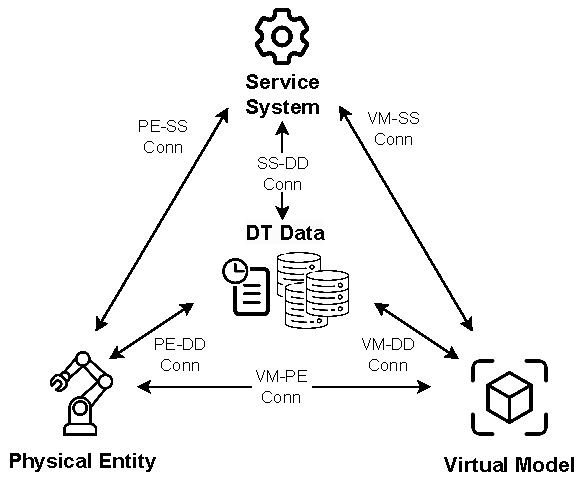
\includegraphics[width=0.6\textwidth]{figures/5d-model.pdf}
    \caption{The 5D model of a Digital Twin.}
    \label{fig:dt-5d-model}
\end{figure}

Tao's 5D model extends Grieves' original model by explicitly including the data and services dimensions, better characterizing the \ac{DT} as a data-driven and service-oriented system. 


The service-oriented nature of \acp{DT} has an essential role in their ability to provide value to users.
%
The \ac{DT} is hence not just a passive representation of a \ac{PA}, but an active system that users can interact with to obtain insights and perform actions on the \ac{PA}.
%
This also contrasts the idea of the \ac{PA}-\ac{DT} system as a closed-loop control system, but rather envisions the \ac{DT} as open to interactions with external entities such as human users or other software systems.

Following this perspective, the idea of \ac{DT}-as-a-service has been proposed.
As shown in \Cref{fig:dt-as-a-service}, the proposed reference architecture adds a cyber layer and an application layer on top of the classic physical, digital and communication layers of a \ac{DT}~\cite{aheleroff2021aei}.
%
The reference architecture further highlights different levels of integration following the taxonomy of Digital Model, Shadow, and Twin~\cite{kritzinger2018dtmanufacturing}, with a further Digital Twin predictive level, which includes predictive models and analytics capabilities enabled by the cyber layer grounded on cloud technologies such as Big Data analytics. 
%
The vision additionally integrates \acp{DT} in an incremental and iterative development lifecycle, to accompany and evolve alongside the \acp{PA} they represent. 

\begin{figure}[ht]
    \centering
    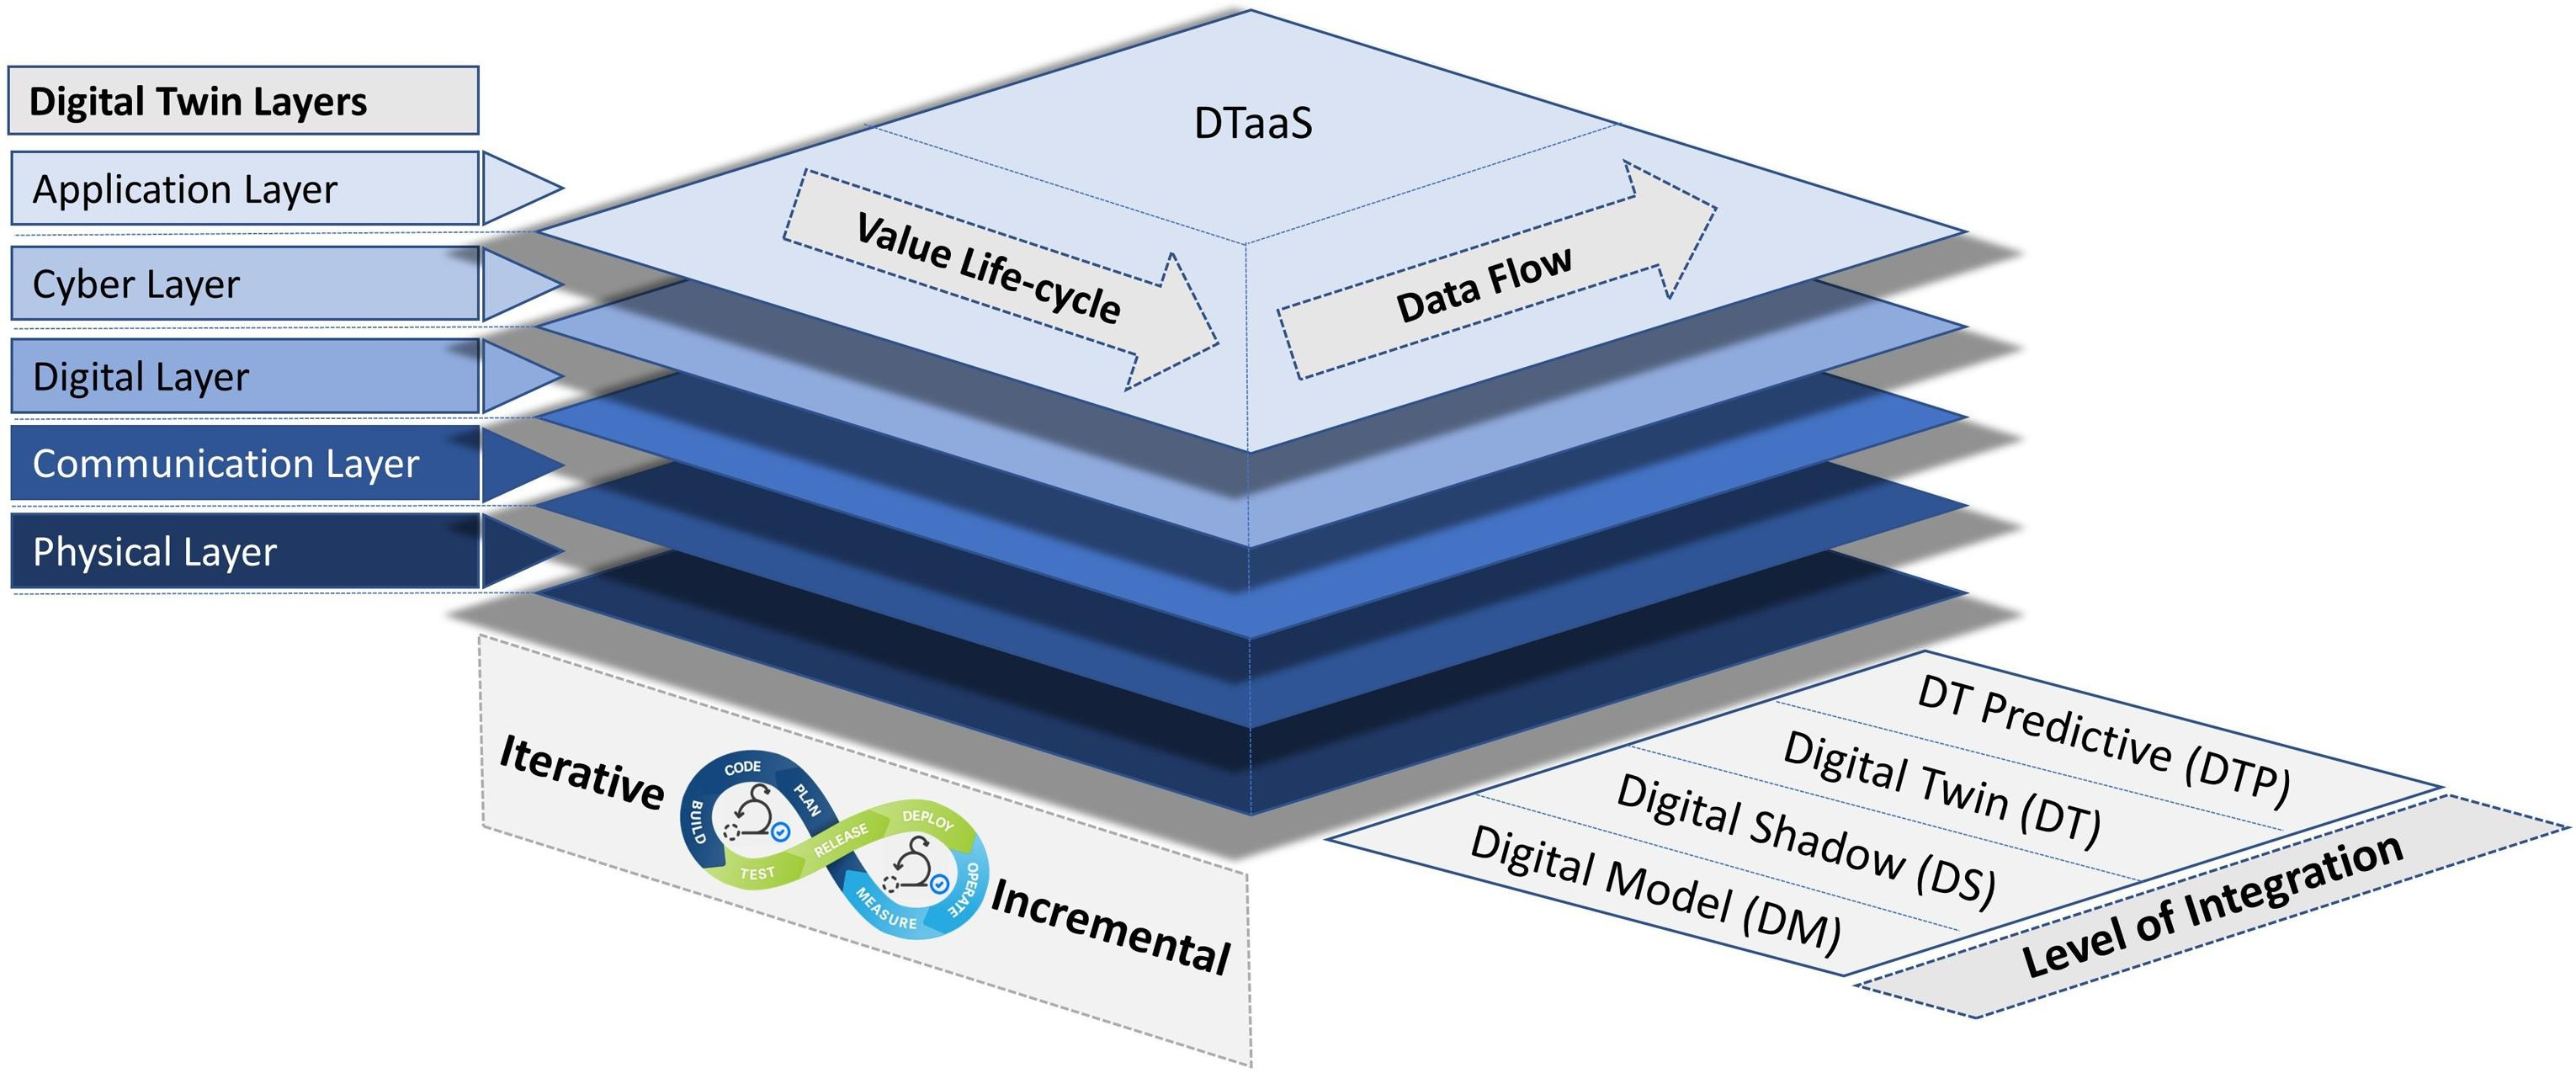
\includegraphics[width=\textwidth]{figures/dt-as-a-service.jpg}
    \caption{The DT-as-a-Service reference architecture, from \cite{aheleroff2021aei}.}
    \label{fig:dt-as-a-service}
\end{figure}

Layered and service-oriented architectures for \acp{DT} are the most popular in the literature.
%
These architectures support desired non-functional quality attributes such as performance efficiency, reliability and maintainability, but also compatibility with existing systems and scalability~\cite{ferko2022architecting}

On the functional side, \cite{dt-IoT-context-Minerva-2020} proposes a set of properties \ac{DT} should have, analyzing existing literature and implementations in the \ac{IoT} context.
%
The properties, summarized in \Cref{tab:minerva-properties} detail various aspects that characterize functional behavior of \acp{DT}.
%
Interestingly, such properties go beyond the generic definition of \ac{DT} as a virtual representation of a \ac{PA} and highlights the various capabilities that a \ac{DT} can provide to its users.

First, both the \ac{DT} and the \ac{PA} are required to be \emph{univocally identifiable} in order to establish a clear relationship between the two. This vision supports the possibility of having possibly multiple \acp{DT} representing the same \ac{PA} in different contexts or for different purposes.
%
Accordingly, the second important contribution is the emphasis on \emph{contextualization}. 
This shifts the focus from the ultra-realistic \ac{DT} envisioned by NASA to a more pragmatic approach where the \ac{DT} is representative of the \ac{PA} in a specific context,
hence possibly abstracting away details of the \ac{PA} that are not relevant for the intended use of the \ac{DT} in the target system.
%
Additional properties emphasize the dynamic nature of the \ac{DT} and its ability to reflect changes in the \ac{PA} (\emph{reflection}), in a timely manner (\emph{entanglement}), persisting over time, memorizing past states and offering a reliable representation of the \ac{PA} (\emph{accountability}). 
%
Finally, the properties also highlight the ability of \acp{DT} to provide value to users through services (\emph{servitization}) such as aggregation of multiple assets (\emph{composability}), augmentation of the \ac{PA} capabilities (\emph{augmentation}), management of access control (\emph{ownership}), and anticipation of future states and behaviors of the \ac{PA} (\emph{predictability}).

\begin{table}[ht]
\centering
\caption{Characterizing Properties of \acp{DT}, defined in \cite{dt-IoT-context-Minerva-2020}.}

\begin{tabular}{p{3.5cm}|p{\dimexpr\textwidth-4.5cm\relax}}
\toprule
\midrule
\textbf{Property} & \textbf{Description} \\
\hline 
\hline
{Contextualization} & A \ac{DT} models the \ac{PA} in a way that is representative with regard to the target context. \\
\hline
{Reflection} & A \ac{DT} reflects changes in the \ac{PA} in real-time. \\
\hline
{Replication} & A \ac{DT} replicates an object into different environments. \\
\hline
{Entanglement} & The degree to which a \ac{DT} is interconnected with its \ac{PA}. \\
\hline
{Persistency} & A \ac{DT} persists over time even when the \ac{PA} is not available. \\
\hline
{Memorization} & A \ac{DT} stores and allows retrieving past states and events. \\
\hline
{Composability} & A \ac{DT} can aggregate different assets or \acp{DT}. \\
\hline
{Accountability} & A \ac{DT} recovers from errors and maintains a reliable state.\\
\hline
{Augmentation} & A \ac{DT} can add new capabilities to the \ac{PA}.\\
\hline
{Ownership} & A \ac{DT} manages access control over its data and functionalities.\\
\hline
{Servitization} & A \ac{DT} provides services to its users.\\
\hline
{Predictability} & A \ac{DT} can anticipate future states and behaviors of the \ac{PA}.\\
\hline
\bottomrule
\end{tabular}%
\label{tab:minerva-properties}
\end{table}



%=======================================================
\section{Technologies and Platforms}
%=======================================================

\note{Enabling Technologies}



\note{The shift from silos to platforms}

\note{Azure DT}

\note{Ditto}

%=======================================================
\section{\aclp{DT} and \acl{AI}}
%=======================================================

\note{This is here to serve the purpose of introducing "Cognitive Digital Twins"
and link to MAS}


%=======================================================
\section{Towards \aclp{DTE}}
%=======================================================

\note{From platforms to ecosystems}

\note{Digital Twin interoperability(?)}

\note{National Digital Twin}

\note{Web of Digital Twins}
